\documentclass[12pt]{article}
\usepackage{cite}
\usepackage{mdframed}
\usepackage{mathrsfs}
\usepackage{graphicx}
\usepackage{caption}
\usepackage{float}
\usepackage{amsmath}
\usepackage{amssymb}

\graphicspath{{../}}

\newenvironment{aside}
  {\begin{mdframed}[style=0,%
      leftline=false,rightline=false,leftmargin=2em,rightmargin=2em,%
          innerleftmargin=0pt,innerrightmargin=0pt,linewidth=0.75pt,%
      skipabove=7pt,skipbelow=7pt]\small}
  {\end{mdframed}}



\begin{document}

\title{Calibrating A Spectrometer Via Global Bayesian Optimization on a Reference Setup}
\author{8241S}
\maketitle

\begin{center}
    \section*{Abstract}
    In this investigation we attempt to create and test a robust software package,
    with the goal to provide calibration for a spectrometer, to be used for exoplanet
    surveying looking for Earth-like planets in HARPS. The proposed technique relies on a
    custom optical setup, used to provide reference light, and the software package to
    be developed, based of Global Bayesian Optimization. The complexity of the 
    algorithms involved, however, proved to require a lot more investigation into 
    optimizing differnt aspects of the process, with no successful example on 
    test simulations. Troughout the investigation, however, a custom numerical integration
    technique was employed and given the large set of possible adjustments to be made to 
    the algorithm used, it is not clear if it is suitable for the problem.
\end{center}

\section{Introduction and Theoretical Background} 
    \subsection{The Problem}

    \subsubsection*{Doppler Method for Exoplanet Survey}
        One of the techniques used for exoplanet surveying is the so-called
        Doppler Method. It relies on the gravitational effect of the planet to 
        be detected on the star, to which it is bound. The elliptical trajectory
        of the planets' orbit causes the parent star to also orbit around their common
        centre of mass. This, in turn, alters the relative speed of the star to the
        Earth, which can be detected via movement of spectral lines of known wavelength,
        most commonly hydrogen lines. The data can be broken down in frequency
        to separate different planets' effect on the parent star. The result is 
        indicative of the properties of the planets in that system in terms of mass 
        and orbit radius and shape. The Doppler Method has been successfully employed 
        in the search of planets, very close to their parent star or of large mass,
        comparable to that of Juputer \cite{exoplanets}. This process, however, requires
        great sensitivity for Earth-like planets, which is why new generation infrastructure,
        such as HARPS are constructed, relying on much more accurate spectrum observations.
        
        \begin{aside}
            The Doppler Effect. 
            
            To demonstrate the requirements on the spectrum 
            measurement we discuss a simplified 2-body system of star and planet of 
            mass ratio $\eta$. Thus we calculate that for observations in the orbital
            plane and for a circular orbit, the unitless doppler shift we expect is:
            \begin{equation}
                \frac{\Delta\lambda}{\lambda} \approx -\frac{v_1}{c}\sqrt{\frac{\eta^2}{(1+\eta)^3}}
            \end{equation}
            Given the orbital speed of the planet, we expect for an Earth-like planet, a value
            of the order of $v_1 \approx 10^{-4}c, \eta \approx 10^{-6}$, thus giving
            the requirement to observe deviations of wavelength of the order of $1$ part in $10^{10}$.
        \end{aside}

    \subsubsection*{Accuracy Requirements For Survey}
        As shown, surveys for Earth-like exoplanets via the Doppler Method, require extreme 
        precision out of the specrtometers used, far exceeding the resolving power of specrtometers
        used today. This project considers the HARPS instrument, with spectral resolution $R = 115'000$.
        However, observations can still be made trough long exposures, wherein the spectra observed
        have a sufficient variation that if a histogram is constructed from neighbouring pixcels as well,
        and probability distribution functions fitted, small variations to the mean of that,
         distribution,
        representing the unmodulated spectral line, can be observed even at a precision level, orders of
        magnitude greater than the resolving power of the instrument. This however requires precise knowledge 
        of the instrument used.

        In particular, such spectrometers use CCD's with finite pixel sizes and sometimes defects in 
        the precise position of the center of the pixels on the CCD. Thus in order to achive the required
        precision, these positions in the spectrum need to be determined. This leads to the need 
        for robust and precise calibration methods.

        An option proposed for determining the pixel positions of a CCD are 
        so-called astro-combs ~\cite{Li_2008}, used to inject light of known spectrum,
        which is to be compared to the observed data from the spectrometer. The light is generated
        with very precise spectrum features, which are also quite narrow, made such trough the use of Fabrý-Perot 
        cavities and custom hardware overall. This yields precision of 1 part in $\approx 10^9$, and is 
        also an extremely expensive methodology. The goal of this investigation is to assess the 
        viability of different, more affordable approaches.

    \subsubsection*{}
    \subsection{Bayesian Optimization Technique}
        Achieving the required calibration precision, without using 
        expensive hardware is generally a tall order. This ivestigations' proposed method 
        for circumventing the need for astro-combs involves a more software-heavy 
        approach. In detail, it involves injecting broadband light from a source of known properties,
        such as a tungsten lamp, trough a Michaelson Interferometer, into the
        spectrometer. This allows interference features to be introduced into
        the light, allowing for a varied spectrum. 

        Calibration is then performed by making intensity measurements,
        and comparing them to a model of the pixel positions, which is to be fitted to the observed light.
        The fitting is to be performed via a global optimization of the parameters, characterizing the model
        used, via Bayesian Optimization.

        This method is well suited to the problem as it is developed for maximization of functions, which
        are expensive to evaluate, as model determination is in this case. The process follows an alogrithm 
        for optmization, described below.

        \begin{aside}
        Summary of Bayesian Optimization. \cite{bo}

        \begin{enumerate}
            \item Model Determination. The first step is to determine an appropriate model and 
            parametrization, along with parameter space, for example given central positions of
            pixels $\mathbf{x}$, on a CCD, which are unperturbed, a model would take the form of: 
            $f(\mathbf{x}, \mathbf{params}) \rightarrow \mathbf{y}$, thus updating the estimates to 
            the vector $\mathbf{y}$. Here a decision of the type of model to be used is important, since
            the Bayesian Optimization algorithm is unsuited for large-dimensional parameter sets,
            so simplifying the number of dimensions of this space is both computationally beneficial and
            a requirement for successful execution.

            \item Set up. The algorithm requires an objective function, which is to be minimized,
            for example the $\chi^2 = \sum_i{\frac{(E_i - O_i)^2}{E_i}}$ value for the model for a given parameter set.
            It also requires a Gaussian Process $\mathscr{GP} = \mathscr{N}(\mu(x), k(x, x'))$, with $\mu(x)$ acting as 
            the current best fit to the model (prior), while the kernel $k(x, x')$ acting as a covariance matrix,
            encapsulating the properties we need to capture. On this step we need to choose appropriate type of kernel, 
            which would capture the desired behaviour of the model in question.

            \item Iterative Step. On each step the algorithm uses the current values of $\mu, k$, derived from
            observations so-far and uses an acquisition function on a random choice of function from $\mathscr{GP}$, taking the process and determining the 
            next point in parameter space to be observed. This is used to construct a posterior distribution, to 
            be used as the next step's pror. Here appropriate choice of acquisition function
            has to be made. There are a number of choices with different qualities. %To summarize those choices and cite

            This step also involves an imporvement of the optimization of the hyperparameters of the problem, 
            for example, the parameters used to define the kernel, such as length-scale $\sigma$ for an Radial Basis Function
            kernel $k(x, x') = \exp{\left(-\frac{\Vert x-x' \Vert^2}{2\sigma^2}\right)}$, commonly used in this process. This is done in order to improve the estimates of $\mu(x)$ in
            following steps.

            \item Finalizing. After a preset number of steps, the algotithm halts and its determined 
            values can be recovered, in order to be used.

        \end{enumerate}
        \end{aside}

\section{Process and Challenges}
    \subsection{Modelling of the required function and set up}
    In order to assess the viability of the method proposed we need a simulation of the 
    setup that is to be used in the actual instrument. To that end, we introduce two factors,
    which contribute to the misallignment of pixels: Randomness and correlation. We produce
    a vector, which is to be found, of the deviation from the proposed centre via a normal
    random number generator, and we then correlate neighbouring pixel deviations spatially.
    The result is illustrated in Fig. \ref{tru_vals}.

    \begin{figure}[H]
        \centering
        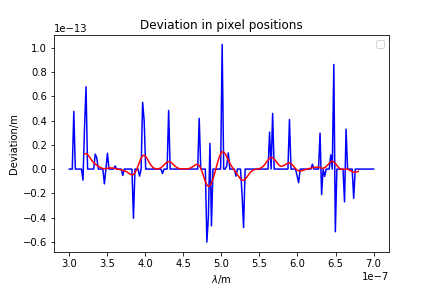
\includegraphics[scale=0.8]{true_vals.png}
        \caption{Simulated deviation in pixel positions, produced to
        be reproduced with a model. Here for simplicity we use 200 pixels
        and use correlation length of 1 pixel. In reality these can be included
        as hyperparameters in a more complex model.}
        \label{tru_vals}
    \end{figure}

    The setup for the procedure then requires an appropriate model, which perturbs the pixel positions,
    The choice of parametrization is very important here as it determines the ability of algorithm to 
    converge reliably. As such there are several possible choices, which were attempted
    in the course of the investigation. In all cases, given computational constraints,
    and the inability of the process to function with a large number of parameters, we 
    resorted to a small number of parameters at leading order.

    \begin{gather}
        \lambda = f(\lambda_0) = \lambda_0 + a + b\lambda_0 + c\lambda^2 + d\lambda^3 + ...\\
        \lambda = f(\lambda_0) = \lambda_0 + a_0 + \sum_{n=1} a_ncos(n k_0\lambda_0) +
        b_nsin(n k_0\lambda_0)
    \end{gather}

    Given this we have models, which can be optimized, and it is then necessary to 
    select parameter space boundaries. Trough running the algorithm, developed, it became
    clear that real challenges to the procedure were presented when too large or too
    small spaces were chosen. In the former case, the algorithm will not explore
    the region of paramters we were interested in (Here the parameter boundaries
    were of the order of $10^2, 10^3$ of the actual parameter values used for testing purposes).
    In the latter case, it is obvious that the exploratory space needs to be greater
    than the actual values, which are to be approached. Thus it was concluded that 
    convergence of the algorithm in a suitable time is only possible given that boundaries
    were preset to around $10$ times the expected outcomes. 


    The next step of producing a working algorithm involves the choice of the 
    so-called objective function. This is utilized by the process to assess the 
    model accuracy to observation. As such we utilized the proposed hardware setup
    for calibration, which we simulated to deduce a global goodness-of-fit. Observations
    consist of simulating the black-body, intensity-normalized spectrum given off by
    a tungsten lamp. This is then passed trough a Michaelson interferometer, which has
    its optical path difference (OPD) calibrated to a satisfactory level of accuracy by 
    trough the use of a reference HeNe Laser and a long delay line \cite{Interferometer}.
    This allowed, as seen on Fig.2 to produce spectra of varying intensity, resulting in 
    a more pronounced change to the error function on deviation.

    \begin{figure}
    \caption{The proposed interferemoter setup and an expected observation.}
    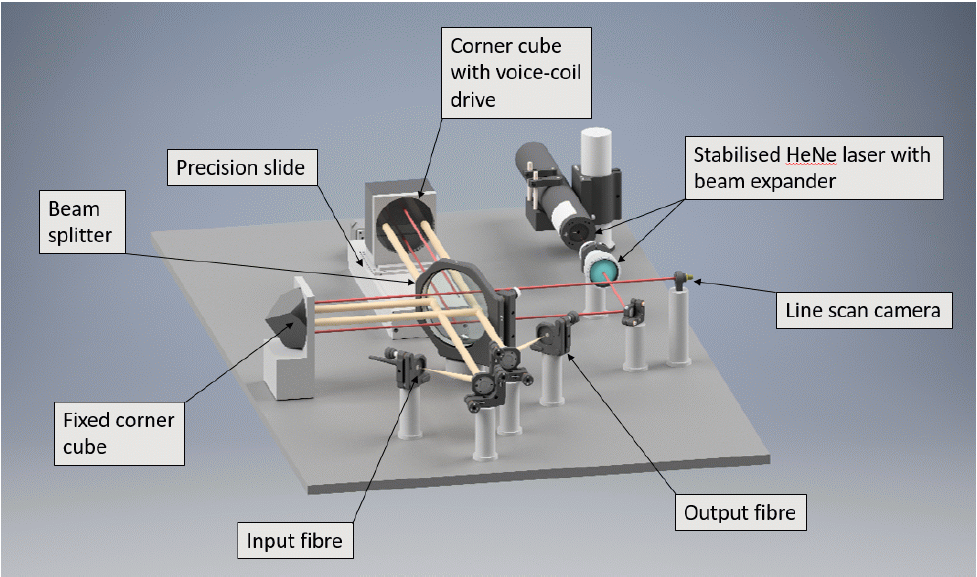
\includegraphics[scale=0.4]{interferometer}
    
\includegraphics[scale=0.35]{test.png}

    \end{figure}
    
     
    \subsection{Challenges with evaluation of the objecticve function}
        The observaitional step, required to determine the goodness-of-fit
        at each step proved to be computationally challenging for a variety 
        of reasons. First, each observation will involve computation of a 
        matrix of the order of $10^9 ~ 10^{10}$ elements. This would be a managable task,
        however the setup as described involves a lot of sources of uncertainty,
        for example, the temperature of the tungsten lamp used in practice. 
        Black-body spectra are sensitive to temperature, and so changes in that 
        parameter would involve a substantial change to the expected, therefore
        modelled spectrum function and so prove the methodology hard to use.

        A technique, we attempted to employ to remedy such sources is a custom 
        numerical integration, targeted at integrals of the type 
        \begin{equation}
            \int_0^\infty f(x)dx
        \end{equation}
        wherein the integrand has a single pronounced maximum. Spceifically in this case, 
        we require for $\mathscr{B}$, being the normalized black-body spectrum
        for temperature $T$, modulated by $\cos(2\pi\frac{x}{\lambda})^2$, from the interferometer,
        and $N$ is a the temperature normal distribution.

        \begin{equation}
            f(T) = \mathscr{B}(T, \lambda, x)\mathscr{N}(T_\mu, T_\sigma)
        \end{equation}
    \begin{aside}
        The integration technique.

        The problem presented with integrals of type in Eq.(4) are related to 
        the sampling required to calculate numerical integrals, used by all methods.
        Most commonly sampling is done linearly, but the upper limit of the integral, 
        requires consideration of the asymptotic behaviour as $x \rightarrow \infty$,
        but also requires that sampling be sufficiently dense within the peak of the function,
        so that its behaviour is accurately captured there. As such linear or even logarithmic
        sampling is not optional. The proposed method involves fitting a normal distribution
        as closely as possible to the integrand, and using it to sample that integrand, with
        sampling being dense within the peak of the function and sparce at the large values off
        the integral, where contributions are small, matching the requirements outlined above.
        The integral is hence calculated via a common methodology for numerical integration
        from samples, here we employ Simpson's technique, given its ease of use
        and relative accuracy. To allow for control over the method we also employ a 
        multiplicative parameter of the standard deviation of the fitted Gaussian, to 
        investigate possible changes to the method accuracy with the spread of the samples. We observed 
        optimal performance around the $10^1, 10^3$ range as displayed by Fig.3. We also observe
        that for low values of the multiplier the integral value is reduced from the true value (the plateu),
        whereas large multiplier values yield significant errors. Thus we get the preferred multiplier of $\approx 10^2$.

    \end{aside}
    \begin{figure}[H]
        \centering
        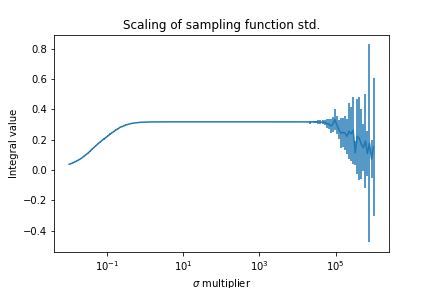
\includegraphics[width=\textwidth]{Integral.png}
        \caption{A display of the effect of the multiplicative paramter on the
        value of an integral of black-body spectra. Here each integration required $10^6$ sample points}
    \end{figure}

    The next step of the algorithm involves the choice of kernel and its parameters, required for
    the purposes of the model, which we need, to be passed to the internal Gaussian Process Regressor.
    Here the choice rest on assumptions about the function in question, such as its differntiability,
    its periodicity, its length scales. As we make no assumtions beside those already in place
    by fixing the form of the model, we use is commonly used, the Mátern kernel \cite{bo}. To this We
    add a White Kernel, used to model noise, which we also later introduce in the observation. Both 
    these kernels come equipped with a set of parameters, which are to be optimized by the internal
    gaussian process regressor used. These are as follows. The Mátern kernel comes with a length scale
    parameter and a $\nu$ parameter, the former encoding the dependence of parameter values 
    on their immediate neighbourhood, the latter encoding the differentiability of the functions to be 
    considered. While, given the information on the shape of function we consider, the length scale 
    was varied less during the investigation, the $\nu$ parameter was varied between the 3 
    starting values of $0.5, 1.5, 2.5$, which are ones, for which analytical, computationally light functions
    were implemented. The White Kernel comes with a noise-level parameter, which was given 
    an initial value of $0$. In all cases the Bayesian Optimization Process implements 
    hyperparameter optimization (The 3 parameters of the kernel mentioned above), trough a process in which
    the regressor assess candidates for possible hyperparameters by evaluating the log-marginal-likelyhood
    for the space given.

    The last step is the choice of acquisition function number of iterations.
    For this investigation, we had the goal of attempting to show that the methodology 
    is useful. To that end we chose 2 common acquisition functions to try: Expected Improvement 
    \cite{bo}, which is more robust, but is very costly to evaluate, and Upper Confidence Bound.
    The latter is realtively easy to evaluate and is known to be able to produce good results.
    Thus more often than not UCB was used, along with parameters which are fixed, 
    which are used to balance the random exploration with guided exploitation of the
    algorithm.

    \subsection{Tests Performed}
    In order to test the viability of the models presented, various tests were 
    performed on a simplified simulation, using an already developed implementation. \cite{bo_impl} \cite{scikit}
    These simulations used reduced pixel sizes (between 200 and 2000) and OPD spaces, in order to more 
    efficiently investigate the effect of different aspects of the algorithm. To investigate the ability of the
    process to converge, tests with set parameters were performed, with 2, 3, 4 or 5
    parameters in the model. As well as this, tests were performed with noisy inputs to
    the spectrum evaluations, varrying the different levels of noise with respect to the
    signal input in the range of $10^{-1}, 10^{-5}$, as well as varying sizes of 
    the parameter spaces. These are values, which were used as they are commonly observed 
    in processess, such as the optical measurements performed here.

    The tests showed no reliable way to get a converging model. No test displays this.
    Further investigations into the parameter function, evaluated on parameter spaces
    revealed that the structure of the objective function is not suitable for the 
    optimization algorithm, as shown in Fig. 4

    Investigation was also attempted a number of times after developing the complete 
    package. This, however, proved fruitless also since computation times for the simulation
    as a whole, generally speaking were found to be of the order of days. This presented 
    a serious challenge to gathering quality data for assessment of the method. 
    \begin{figure}
        \centering
        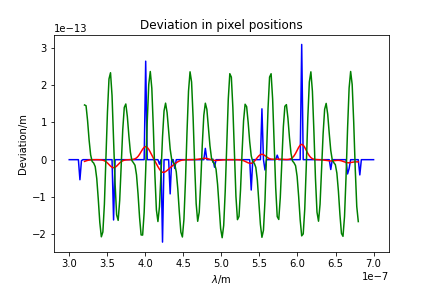
\includegraphics[scale=0.4]{fit.png}
        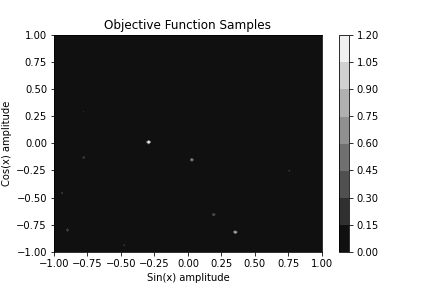
\includegraphics[scale=0.4]{Sinusoid_objective_func (2).png}
        \caption{Tests performed in order to evaluarte the objective function
        responsiveness and the model(red line is actual values, green line is the model) fit after 130 iterations.}
    \end{figure}
\section{Discussion}
    The failiure to produce any reasonably convergent algorithm might indicate that
    this methodology is not optimal for the problem at hand. However such strong
    conclusion cannot be drawn from this investigation alone, given the time and resource
    constraints. It is possible that a greater amount of time needs to be allocated 
    to parallalizing the software, built for the simulations, allowing for a 
    much more comprehensive read of the possibilities. This, however, comes with its 
    set of challenges, such as the difficulty of performing that task and also there 
    are limitations such as the floating point format used to pass to parallel systems. 
    Another possibility is that the models attempted were not suitable for this test. A more in-depth
    analysis would be required to determine a better strategy for the calibration.
\bibliographystyle{plain}
\bibliography{ref}{}

\end{document}